\documentclass[../main-report.tex]{subfiles}
\begin{document}
\section{Giới thiệu}
Mã hóa đầu cuối (\acrshort{e2e}) là một dạng mã hóa dữ liệu đầu cuối đối với những tin nhắn chat, thư email được gửi và trao đổi trên Internet. \acrshort{e2e} đang trở thành tiêu chuẩn cho các ứng dụng nhắn tin. WhatsApp là một ví dụ nổi bật, với hàng tỷ người dùng. Tất cả những trao đổi trực tiếp trên ứng dụng đó đều được mã hóa bảo vệ như: “Tin nhắn, hình ảnh, cuộc gọi, video, âm thanh, và một vài tệp tin đính kèm khác”.

Mã hóa đầu cuối cải thiện sự riêng tư của người dùng bằng cách làm cho tin nhắn không thể đọc được cho bất kỳ ai ngoài người nhận dự định của họ. Đặc biệt, tin nhắn không thể đọc được từ máy chủ nhắn tin. Điều này làm giảm \gls{Trusted Computing Base} và bảo vệ chống lại khả năng máy chủ có thể bị xâm phạm, ví dụ như nhân viên lừa đảo, tin tặc hoặc cơ quan giám sát. Các sự kiện trong thế giới thực cho thấy sự thỏa hiệp của máy chủ là mối đe dọa hợp pháp, bao gồm cả việc truy cập hàng loạt NSA vào các công ty Internet dữ liệu qua PRISM [\cite{7}] và bằng chứng về việc nhân viên truy cập dữ liệu không phù hợp tại Facebook [\cite{8}] và Snap [\cite{9}].

\begin{figure}[ht!]
\begin{center}
\label{fig:E2E}
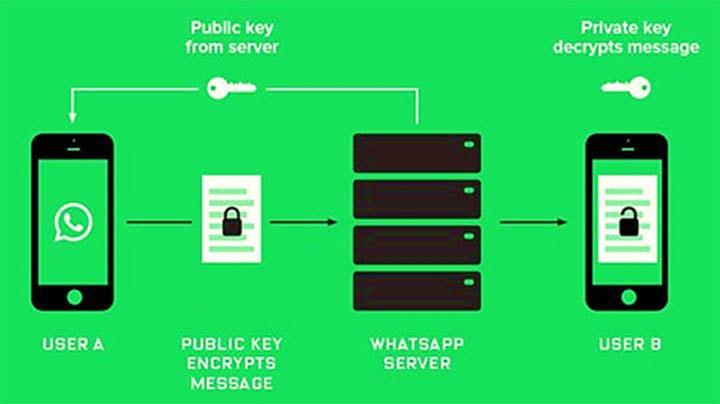
\includegraphics[scale=0.65]{E2EApp}
\caption{Mã khóa riêng tư tin nhắn trong ứng dụng Whatsapp}
\end{center}
\end{figure}

Tiện ích mới cho người dùng các ứng dụng là có 2 giao diện mã khóa: mã khóa công khai và mã khóa riêng tư. Khóa công khai sẽ cho phép mọi người nhìn thấy thông tin dữ liệu trao đổi, và đăng tải lên đám mây Google. Ngược lại, khóa riêng tư thì chỉ cho phép người nhận và người gửi xem thông tin nội dung dữ liệu truyền tải, không cho bất kỳ bên thứ 3 nào tham gia quá trình trao đổi này. Mọi thông tin bảo mật đều được khóa riêng tư lưu trữ trên trình duyệt. Để nâng cấp thêm tính năng này, cho phép người dùng có thể điều chỉnh thiết lập lại thời gian chờ của tin nhắn, gia hạn lưu trữ các tin nhắn đến, tự động xóa các tin nhắn cũ, theo quy định số lượng tin nhắn hay thời gian tin nhắn ra khỏi bộ nhớ hệ thống. Cũng có thể lưu trữ một lượng lớn tin nhắn.


\section{Tổng quan Secure Two-party Messaging}
\label{sec:related-work}
Trong mục này, chúng tôi mô tả ngắn gọn trường hợp đơn giản hơn về nhắn tin hai bên an toàn. Chúng tôi cũng nêu rõ những khó khăn khi chuyển sang nhắn tin nhóm an toàn. Chúng tôi sẽ giới thiệu các khái niệm mật mã làm nền cho các chương sau.

Mục tiêu cơ bản của nhắn tin bảo mật hai bên là cho phép hai người dùng có một cuộc trò chuyện an toàn. Bảo mật trong bối cảnh này có nhiều phần. \gls{Confidentiality} (\glsdesc{Confidentiality})là thuộc tính mà chỉ có hai người tham gia có thể biết được tin nhắn plaintext. \gls{Integrity} (\glsdesc{Integrity}) là thuộc tính mà chỉ hai người tham gia mới có thể gửi tin nhắn, tức là, những người tham gia sẽ từ chối các tin nhắn đã được gửi hoặc giả mạo bởi người ngoài. \gls{Authentication} (\glsdesc{Authentication}) là thuộc tính mà hai người tham gia đồng ý về các danh tính của nhau, thường được biểu thị bằng các khóa công khai.

Các thuộc tính này thường được đo dựa trên hacker, có thể đọc và lưu trữ tất cả các liên lạc giữa các bên, gửi tin nhắn giả mạo và bắt đầu các cuộc hội thoại an toàn, tuân theo giới hạn thực tế về sức mạnh tính toán của nó.

Mã hóa bất đối xứng, như trong \acrshort{pgp}, đạt được các thuộc tính trên chống lại một hacker. Tuy nhiên, nó không đạt được các đặc tính bảo mật nâng cao về bảo mật bí mật và bảo mật sau thỏa hiệp, được đo lường trước một kẻ thù cũng có thể thỏa hiệp với người dùng, đang học tất cả các khóa bí mật của họ tại một thời điểm nhất định.

\gls{Forward secrecy} (\glsdesc{Forward secrecy}) là thuộc tính mà một hacker thỏa hiệp một số hoặc tất cả người dùng sẽ không thể giải mã tin nhắn từ trước khi thỏa hiệp. Có thể đạt được bí mật về mức độ chi tiết của toàn bộ các cuộc hội thoại cùng với các thuộc tính trên bằng cách sử dụng trao đổi Diffie-Hellman đã được xác thực để thiết lập khóa chia sẻ tồn tại ngắn và mới (không được sử dụng trước đó) cho mỗi cuộc hội thoại, sau đó mã hóa tin nhắn theo khóa sử dụng sơ đồ mã hóa xác thực với dữ liệu liên kết (\acrshort{aead}) [\cite{10}], như trong \acrshort{tls-dhe} [\cite{11}]. Bảo mật chuyển tiếp ở mức độ chi tiết của các thông điệp riêng lẻ có thể đạt được bằng cách sử dụng thêm tính năng ghép mã khóa xác định, được giới thiệu bởi SCIMP [\cite{12}]. Theo cách tiếp cận này, người dùng mã hóa mọi tin nhắn bằng một khóa duy nhất, xuất phát từ một số khóa được chia sẻ bằng cách sử dụng chuỗi ứng dụng hàm băm và xóa khóa ngay sau khi sử dụng.

\gls{Post-compromise security} (\glsdesc{Post-compromise security}), còn được gọi là bảo mật ngược hoặc tự phục hồi, là thuộc tính mà hacker tạm thời thỏa hiệp một số hoặc tất cả người dùng không thể giải mã tin nhắn vô thời hạn sau khi thỏa hiệp được phục hồi. Điều này hữu ích trong trường hợp đối thủ tạm thời truy cập thiết bị và tạo một bản sao trạng thái của thiết bị, ví dụ như thông qua phần mềm độc hại hoặc kiểm tra vật lý, nhưng sau đó mất quyền truy cập vào thiết bị. Bảo mật sau thỏa hiệp có thể đạt được bằng cách liên tục làm mới khóa chia sẻ tồn tại ngắn bằng cách sử dụng các trao đổi Diffie-Hellman mới, một kỹ thuật được giới thiệu bởi OTR [\cite{13}].

Tất cả các thuộc tính trên đều đạt được bằng giao thức two-party Signal [\cite{14,15}], được sử dụng cho các cuộc hội thoại hai bên trong Signal và WhatsApp. Giao thức Signal không đồng bộ ở chỗ người dùng có thể gửi tin nhắn khi người dùng khác ngoại tuyến, sử dụng máy chủ lưu trữ và chuyển tiếp để đệm tin nhắn. Điều này đúng ngay cả với tin nhắn đầu tiên trong một cuộc trò chuyện: bằng cách tải xuống một người dùng khác làm con mồi từ một máy chủ không tin cậy, người dùng có thể thiết lập một khóa chia sẻ tồn tại ngắn xác thực mà không cần giao tiếp. Ở đây một con mồi (prekeys) là thông điệp đầu tiên của một cuộc trao đổi Diffie-Hellman đã được chứng thực; mỗi người dùng tải lên trước một số con mồi cho một máy chủ không tin cậy, để những người dùng khác sau đó có thể sử dụng chúng để hoàn thành trao đổi Diffie-Hellman và bắt đầu một cuộc trò chuyện ngay lập tức. Giao thức Signal cũng đạt được thuộc tính từ chối, điều này nói rõ rằng một người dùng không thể chứng minh bằng mật mã rằng người dùng kia đã gửi bất kỳ tin nhắn cụ thể nào.


\section{From Two Parties to a Group}

Chuyển từ cài đặt hai bên sang các nhóm kích thước tùy ý đưa ra những thách thức mới. Một cách tiếp cận đơn giản để đạt được các thuộc tính bảo mật trên là cho người dùng gửi tin nhắn nhóm qua các kênh giao thức Signal riêng biệt cho từng người dùng, như trong các cuộc trò chuyện nhóm Signal [\cite{16}]; tuy nhiên, điều này không hiệu quả, vì người gửi phải mã hóa và gửi từng tin nhắn một lần cho mỗi thành viên nhóm. Đạt được các thuộc tính như bảo mật sau thỏa hiệp trong khi vẫn cho phép truyền phát thông điệp là một thách thức không cần thiết.

Ngoài ra, việc cài đặt nhóm sẽ thêm các thuộc tính bảo mật mong muốn mới. Xác thực tác giả là thuộc tính mà người dùng có thể xác minh ai đã gửi một tin nhắn cụ thể. Tính toàn vẹn và xác thực ngụ ý rằng người dùng luôn biết rằng một số thành viên nhóm dự định đã gửi tin nhắn, nhưng không giống như trong trường hợp hai bên, họ không biết đó là thành viên nhóm nào, ngoại trừ đó là ai đó ngoài chính họ. Tính nhất quán là thuộc tính mà tất cả người dùng đồng ý về những gì đang xảy ra trong nhóm. Điều này bao gồm tính nhất quán của người tham gia, trong đó tất cả người dùng đồng ý về nhóm thành viên nhóm và tính nhất quán của bảng điểm, trong đó tất cả người dùng đồng ý về nhóm thư được gửi cho đến nay và thứ tự của họ. Lưu ý rằng các hacker cho các thuộc tính này có thể bao gồm các thành viên nhóm độc hại, những người có thể cố gắng giả mạo các tác giả tin nhắn hoặc phá vỡ tính nhất quán của người dùng khác, ngoài các hacker, có thể bao gồm cả máy chủ.

Trật tự tin nhắn cũng khó khăn hơn trong cài đặt nhóm. Thông thường, các ứng dụng nhắn tin hiển thị tin nhắn theo thứ tự tuyến tính. Tuy nhiên, khi có nhiều hơn hai người dùng, thật khó để thực thi một trật tự tuyến tính nhất quán mà không có máy chủ trung tâm và không phải tất cả các ứng dụng đều yêu cầu một thứ tự tuyến tính. Vì vậy, chúng tôi cũng xem xét hai thứ tự yếu hơn. Thứ tự trước sau là thứ tự từng phần trong đó m đứng trước m’ nếu tác giả của m nhận và xử lý m trước khi gửi m’. Điều này bao gồm trường hợp m và m’ có cùng tác giả và m được gửi trước m’. Thứ tự trước sau chính xác là những gì CRDT yêu cầu: để thiết lập trạng thái chia sẻ nhất quán, tất cả người dùng phải nhận tin nhắn theo thứ tự trước sau nhất quán, nhưng họ không cần nhận tin nhắn theo cùng một thứ tự tuyến tính [\cite{17}]. Chúng tôi cũng định nghĩa thứ tự cho mỗi người gửi là thứ tự từng phần trong đó m đứng trước m’ nếu m và m’ có cùng tác giả và tác giả đã gửi m trước m’.

\section{Kiến thức nền tảng}
\subsection{Giao thức Messaging Layer Security (MLS)}

Mục tiêu của giao thức này là cho phép một nhóm người tham gia trao đổi tin nhắn bí mật và xác thực. Bằng cách lấy ra một chuỗi các bí mật và \glsdesc{key} chỉ được biết bởi các thành viên nhóm. Điều này nên được giữ bí để mật chống lại một kẻ thù mạng và nên giữ bí mật cả về phía trước và sau thỏa hiệp đối với sự thỏa hiệp của người tham gia.

Chúng tôi mô tả thông tin được lưu trữ bởi mỗi client là \_state\_, bao gồm cả dữ liệu công khai và riêng tư. Trạng thái ban đầu được thiết lập bởi người tạo nhóm, đó là một nhóm chỉ chứa chính họ. Sau đó, người tạo sẽ gửi các yêu cầu \_Add\_ cho mỗi client trong nhóm thành viên ban đầu, theo sau là thông báo \_Commit\_ kết hợp tất cả \_Adds\_ vào trạng thái nhóm. Cuối cùng, người tạo nhóm tạo ra một thông báo \_Welcome\_ tương ứng với \_Commit\_ và gửi trực tiếp thông báo này đến tất cả các thành viên mới, những người có thể sử dụng thông tin chứa trong đó để thiết lập trạng thái nhóm của riêng họ và lấy bí mật chung. Thành viên trao đổi thông điệp \_Commit\_ bảo mật sau thỏa hiệp, để thêm thành viên mới và xóa thành viên hiện có. Các thông điệp này tạo ra các bí mật được chia sẻ mới có mối liên hệ nhân quả với người tiền nhiệm của chúng, tạo thành một \glsdesc{Directed Acyclic Graph} (\acrfull{dag}) hợp lý. 

Các thuật toán giao thức chúng tôi chỉ định ở đây. Mỗi thuật toán chỉ định cả (i) cách một client thực hiện thao tác và (ii) cách các client khác cập nhật trạng thái của họ dựa trên nó:

\begin{itemize}
\item{Thêm một thành viên, được khởi xướng bởi một thành viên hiện tại.}
\item{Cập nhật bí mật của một thành viên.}
\item{Xóa một thành viên.}
\end{itemize}

Mỗi thao tác này được "yêu cầu" bằng cách gửi tin nhắn thuộc loại tương ứng (\glsdesc{Add} / \glsdesc{Update} / \glsdesc{Remove}). Tuy nhiên, trạng thái của nhóm không được thay đổi cho đến khi một thông báo \glsdesc{Commit} được gửi để cung cấp cho nhóm với thông tin ngẫu nhiên mới. Trong phần này, chúng tôi cho thấy mỗi yêu cầu được cam kết ngay lập tức, nhưng trong các trường hợp triển khai nâng cao hơn, một ứng dụng có thể thu thập một số yêu cầu trước khi thực hiện tất cả các yêu cầu cùng một lúc.

Trước khi khởi tạo một nhóm, client công khai InitKeys (dưới dạng đối tượng KeyPackage) vào một thư mục được cung cấp bởi \glsdesc{Messaging Service}.

\begin{figure}[!h]
\begin{center}
\label{fig:Add}
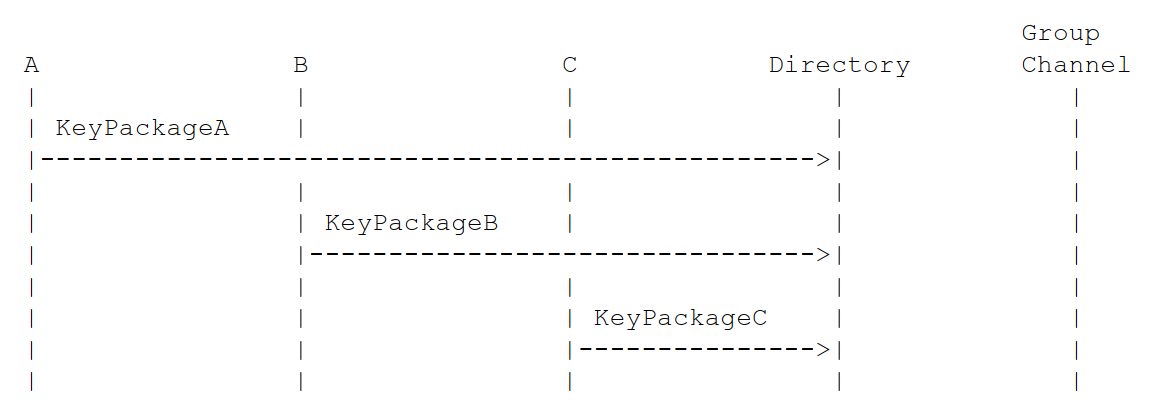
\includegraphics[scale=0.65]{Add1}
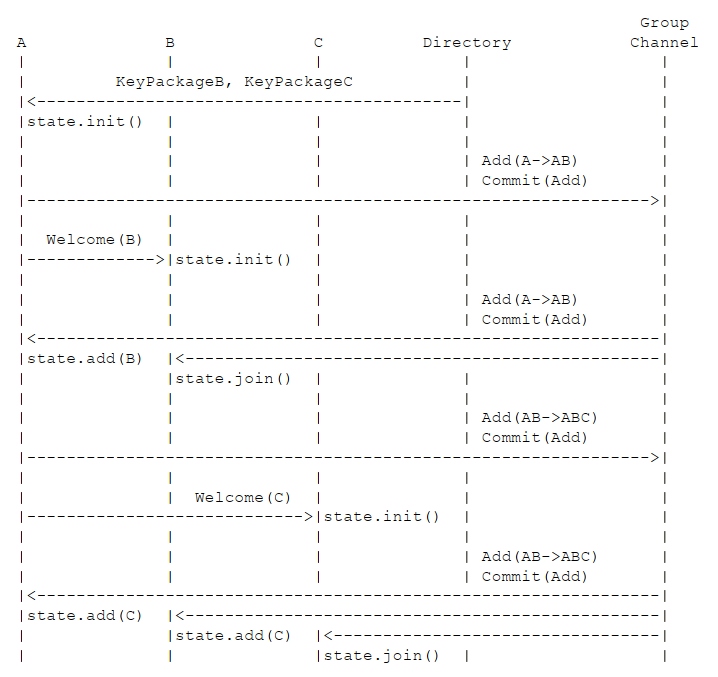
\includegraphics[scale=1]{Add2}
\caption{Quy trình thêm Client vào nhóm}
\end{center}
\end{figure}

Khi client A muốn thiết lập một nhóm với B và C [Hình ~\ref{fig:Add}], trước tiên, nó tải xuống KeyPackages cho B và C. Sau đó, nó khởi tạo trạng thái nhóm chỉ chứa chính nó và sử dụng KeyPackages để tính toán Welcome và Add messages để thêm B và C, trong một trình tự được chọn bởi A. Các Welcome messages được gửi trực tiếp đến các thành viên mới (không cần gửi chúng đến nhóm). Các Add messages được gửi đến nhóm và được xử lý theo trình tự bởi B và C. Tin nhắn nhận được trước khi client tham gia nhóm sẽ bị bỏ qua. Chỉ sau khi A nhận được Add messages từ máy chủ, nó mới cập nhật trạng thái để phản ánh sự bổ sung của họ.

Việc bổ sung các thành viên nhóm sau đó được tiến hành theo cách tương tự. Bất kỳ thành viên nào trong nhóm đều có thể tải xuống KeyPackage của client mới và phát thông báo Add message mà nhóm hiện tại có thể sử dụng để cập nhật trạng thái của họ và Welcome message mà client mới có thể sử dụng để khởi tạo trạng thái của mình.

Để thực thi bảo mật về trước và sau thỏa hiệp, mỗi thành viên định kỳ cập nhật bí mật của họ [Hình ~\ref{fig:update}] . Bất kỳ thành viên nào cũng có thể cập nhật thông tin này bất cứ lúc nào bằng cách tạo KeyPackage mới và gửi Update message theo sau là Commit message. Một khi tất cả các thành viên đã xử lý xong, các bí mật của nhóm sẽ không được biết đến kể cả với kẻ tấn công đã xâm phạm bí mật trước của người gửi. 

\begin{figure}[!h]
\begin{center}
\label{fig:update}
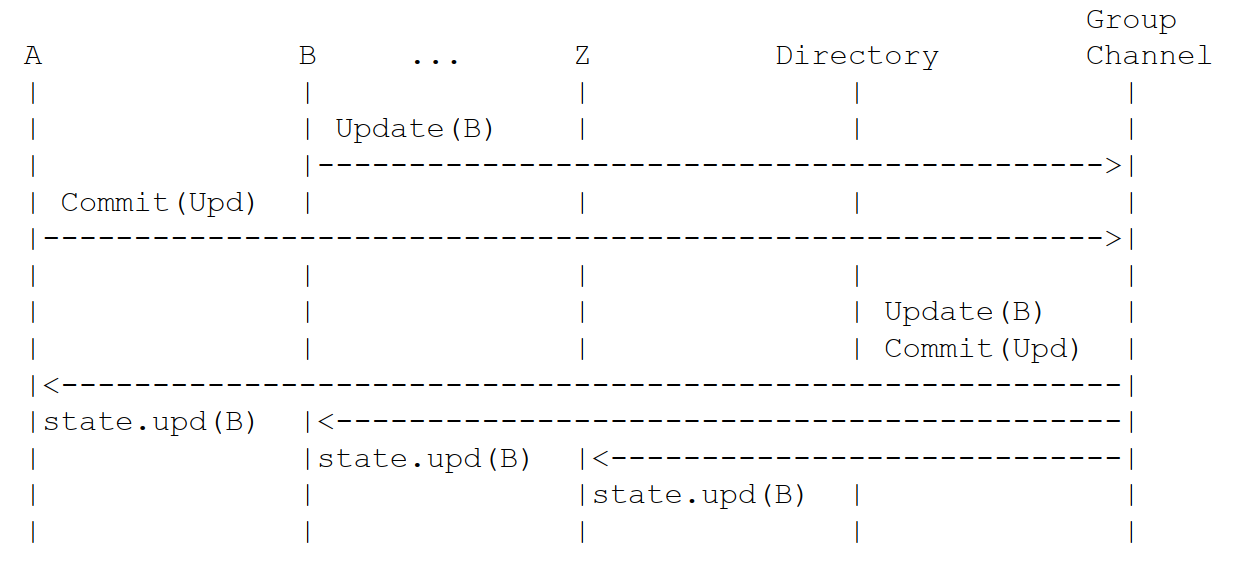
\includegraphics[scale=0.65]{Update}
\caption{Quy trình cập nhật key của nhóm}
\end{center}
\end{figure}

Nó được ứng dụng sử dụng để xác định một chính sách thường xuyên gửi Update message. Chính sách này có thể mạnh như yêu cầu Update + Commit sau mỗi thông báo ứng dụng hoặc yếu hơn, chẳng hạn như mỗi giờ, ngày,… một lần. 

\begin{figure}[!h]
\begin{center}
\label{fig:remove}
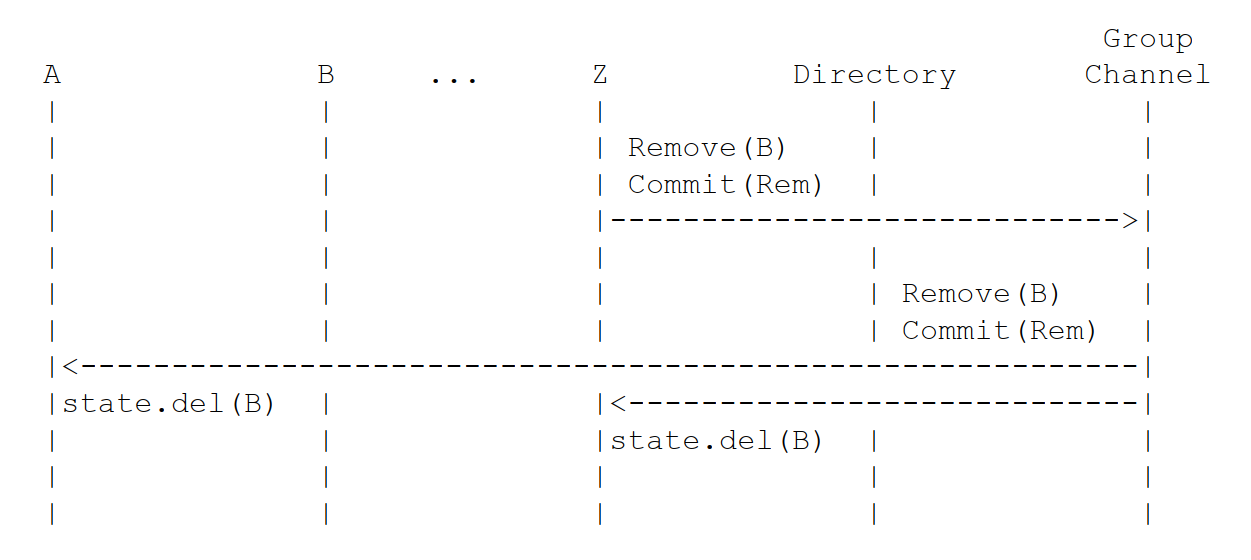
\includegraphics[scale=0.65]{Remove}
\caption{Quy trình xóa thành viên nhóm}
\end{center}
\end{figure}

Các thành viên bị xóa khỏi nhóm theo cách tương tự [Hình ~\ref{fig:remove}]. Bất kỳ thành viên nào trong nhóm đều có thể gửi yêu cầu \gls{Remove} theo sau là thông báo \gls{Commit}, bổ sung thông tin ngẫu nhiên mới cho trạng thái nhóm mà tất cả mọi người biết, ngoại trừ thành viên bị xóa. Lưu ý rằng điều này không nhất thiết ngụ ý rằng bất kỳ thành viên nào thực sự được phép xóa các thành viên khác; các nhóm có thể thực thi các chính sách kiểm soát truy cập trên cơ chế cơ bản này.



\section{Ratchet Tree}
Giao thức sử dụng thuật toán "ratchet trees" để lấy bí mật chung giữa một nhóm client.

\subsection{Thuật ngữ tính toán trong cây}
Cây bao gồm \_nodes\_. Một nút là một \_leaf\_ nếu nó không có con và \_parent\_ nếu có; lưu ý rằng tất cả các nút cha trong cây của có chính xác hai con, một \_left\_ và một \_right\_. Một nút là \_root\_ của cây nếu nó không có cha và \_intermediate\_ (trung gian) nếu nó có cả con và bố mẹ. \_Descendants\_ của một nút là nút đó, con của nó và con cháu của các con của nó và chúng ta nói một cây \_contains\_ một nút nếu nút đó là con của nút gốc. Các nút là \_siblings\_ nếu chúng có cùng cha mẹ.

Một \_subtree\_ của một cây là cây được đưa ra bởi con cháu của bất kỳ nút nào, là \_head\_ của cây con. \_Size\_ của cây hoặc cây con là số nút lá mà nó chứa. Đối với một nút cha bất kỳ, \_left subtree\_ của nó là cây con lấy nút con bên trái của nó làm gốc (tương ứng là \_right subtree\_).

Tất cả các cây được sử dụng trong giao thức này là \glsdesc{left-balanced binary trees} (\gls{left-balanced binary trees}). Cây nhị phân là \_full\_ (và \_balanced\_) nếu kích thước của nó là lũy thừa của hai và đối với bất kỳ nút cha nào trong cây, các cây con trái và phải của nó có cùng kích thước. Nếu một cây con là \_full\_  và nó không phải là một tập hợp con của bất kỳ cây con đầy đủ khác, thì được gọi là \_maximal\_. 

Cây nhị phân là \_left-balanced\_ nếu với mỗi nút cha, thì nút cha này được cân bằng hoặc cây con bên trái của nút cha đó là cây con đầy đủ lớn nhất có thể được xây dựng từ các lá có trong cây con của nút cha. Đưa ra một danh sách các mục "n", có một cây nhị phân cân bằng trái duy nhất với các phần tử này là các lá. Trong một cây cân bằng bên trái như vậy, nút lá "k-th" đề cập đến nút lá "k-th" trong cây khi đếm từ bên trái, bắt đầu từ 0.

\_direct path\_ của một nút gốc là danh sách bất kỳ nút nào là sự kết hợp của nút cha đó cùng với đường dẫn trực tiếp đến nút cha đó. \_copath\_ của một nút là anh chị em của nút được nối với danh sách anh chị em của tất cả các nút trong đường dẫn trực tiếp của nó. [Hình ~\ref{fig:Ratchet-tree}]

\begin{figure}[!h]
\begin{center}
\label{fig:Ratchet-tree}
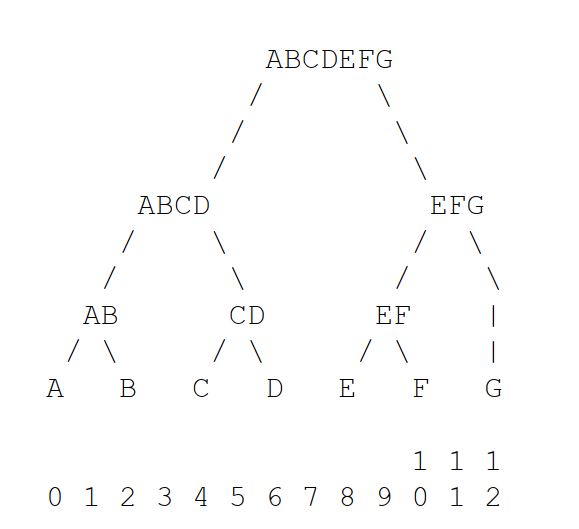
\includegraphics[scale=0.65]{Ratchet tree}
\caption{Direct path của C là (CD, ABCD, ABCDEFG).}

{Copath của C là (D, AB, EFG).}
\end{center}
\end{figure}

Mỗi nút trong cây được gán một \_node index\_, bắt đầu từ 0 và chạy từ trái sang phải. Một nút là một nút lá khi và chỉ khi nó có một chỉ số chẵn. Các chỉ số nút cho các nút trong cây trên như sau:
0 = A ; 1 = AB ; 2 = B ; 3 = ABCD ; 4 = C ; 5 = CD ; 6 = D ; 7 = ABCDEFG ; 8 = E ; 9 = EF ; 10 = F ; 11 = EFG ; 12 = G

Các lá của cây được lập chỉ mục riêng, sử dụng \_leaf index\_, vì các thông điệp giao thức chỉ cần tham chiếu đến các lá trong cây. Giống như các nút, lá được đánh số từ trái sang phải. Lưu ý rằng với cách đánh số ở trên, một nút là một nút lá khi và chỉ khi nó có một chỉ số nút chẵn và một nút lá có chỉ số của nút là một nửa chỉ số nút cha của nó. Các chỉ số lá trong cây trên như sau:
0 = A ; 1 = B ; 2 = C ; 3 = D ; 4 = E ; 5 = F ; 6 = G

Mỗi nút, bất kể nút đó là trống hay không, đều có \_hash\_ tương ứng chứa các thông tin tóm tắt của nút con bên dưới nút đó


\subsection{Ratchet Tree Nodes}
Một phiên bản cụ thể của ratchet tree dựa trên các nguyên hàm mã hóa sau, được xác định bởi mật mã đang sử dụng:

\begin{itemize}
\item{Một mật mã HPKE, chỉ định \glsdesc{KEM} \acrfull{kem}, sơ đồ mã hóa \acrshort{aead} và hàm băm.}
\item{Hàm \acrfull{dkp} tạo ra cặp khóa bất đối xứng cho \acrshort{kem} được chỉ định từ một bí mật đối xứng.}
\end{itemize} 

Mỗi nút trong cây ratchet chứa các giá trị mặc định sau:

\begin{itemize}
\item{Khóa bí mật}
\item{Khóa công khai}
\item{Tên nút}
\item{ID nút}
\item{node secret}
\end{itemize}

\section{Basic background on TreeKEM}
Mỗi người dùng biết tất cả các bí mật nút trên đường dẫn đến lá của họ, cũng như tất cả các khóa công khai trong cây, nhưng họ không thể tính toán các bí mật nút khác trong cây.

Một hàm \acrfull{dkp} ánh xạ các chuỗi nhị phân thành các cặp khóa bất đối xứng (\gls{Private key}; \gls{Public key}).

\begin{itemize}
\item{(\gls{Private key}; \gls{Public key}) = \acrshort{dkp}(node secret)}
\end{itemize}

Hàm \acrfull{kdf} ánh xạ các cặp nhị phân của chuỗi nhị phân thành chuỗi nhị phân, mà chúng ta coi là hàm băm hai đầu vào chống va chạm (Collision resistance)

\begin{itemize}
\item{Collision resistance là một thuộc tính của hàm băm mật mã: hàm băm H có khả năng chống va chạm nếu khó tìm thấy hai đầu vào băm cho cùng một đầu ra; nghĩa là, hai đầu vào a và b sao cho H(a) = H(b) và a $\neq$ b}
\item{Sử dụng KDF để tạo 1 secret mới từ secret cũ: (secret 2) = KDF((secret 1); "next")}
\end{itemize}

Mỗi nút có 3 giá trị:

\begin{itemize}
\item{Node secret}
\item{\gls{Public key}}
\item{\gls{Private key}}
\end{itemize}

\begin{figure}[!h]
\begin{center}
\label{fig:tree}
\includegraphics[scale=1]{tree}
\caption{Một cây ratchet có bốn người dùng A, B, C, D}

{Ở đây chúng tôi hiển thị các bí mật nút tại mỗi nút}
\end{center}
\end{figure}

\newpage
\subsection{Key Update}
Bất cứ lúc nào, bất kỳ người dùng nào cũng có thể thực hiện cập nhật khóa bằng cách gửi tin nhắn \gls{Update}. Điều này thay thế một số bí mật nút trong cây, bao gồm cả bí mật nút gốc. Cập nhật khóa là rất quan trọng để đạt được bảo mật về phía trước và bảo mật sau thỏa hiệp.

Để thực hiện cập nhật khóa, người dùng U đầu tiên tạo ra một bí mật mới x

Sau đó người dùng U, tạo path secret cho nó và các nút trong đường dẫn trực tiếp của nó
\begin{itemize}
	\item{path secret của nút lá U là: x}
	\item{path secret của nút cha của 1 nút là L: = \acrshort{kdf}(path secret của L; "path")}
\end{itemize}
	%\item{Sau đó, đối với mỗi nút này, A cập nhật bản sao của cây ratchet bằng cách cài đặt}
Sau đó người dùng A cập nhật bí mật nút của nó và các nút liên quan
\begin{itemize}
	\item{node secret của nút L: = \acrshort{kdf}(path secret của L, "node")}
\end{itemize}

Lưu ý rằng các path secret là các giá trị tạm thời chỉ được sử dụng trong quá trình cập nhật khóa; chỉ các node secret trở thành một phần của trạng thái được lưu trữ. [Hình ~\ref{fig:path-secret}] cho thấy quá trình phát sinh bí mật ở dạng sơ đồ, trong khi [Hình ~\ref{fig:Update-tree}] cho thấy hiệu ứng của một cập nhật ví dụ U = A trong một cây có bốn người dùng.

\begin{figure}[!h]
\begin{center}
\label{fig:path-secret}
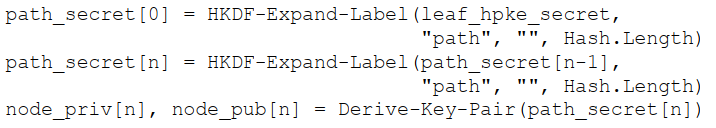
\includegraphics[scale=1]{path-secret}
\caption{node secrets x$_{1}^{N}$; x$_{2}^{N}$; x$_{3}^{N}$ và path secrets x$_{1}^{P}$; x$_{2}^{P}$; x$_{3}^{P}$ từ nút lá đến nút gốc}
\end{center}
\end{figure}

Sau khi cập nhật các bí mật nút ở trạng thái riêng như trên, U gửi thông báo \gls{Update} cho nhóm để thông báo cho họ về những thay đổi này, để nhóm duy trì một cây ratchet dùng chung. Thông báo \gls{Update} chứa:

\begin{enumerate}
	\item{Đối với mỗi nút L trên đường dẫn trực tiếp của U, khóa công khai mới cho L, tức là, pub (node secret mới cho L). Trong ví dụ của [Hình ~\ref{fig:Update-tree}], các khóa công khai này là pub (x$_{1}^{N}$) cho nút lá A và pub x$_{2}^{N}$ cho cha mẹ của A và B.}
	\item{Đối với mỗi nút M trên đường dẫn dán tiếp U, bí mật đường dẫn mới cho cha mẹ M, được mã hóa không đối xứng dưới các khóa chung của mỗi nút. Trong ví dụ của [Hình ~\ref{fig:Update-tree}], các mã hóa này là \textit{Enc$_{pub(b)}$(x$^{P}_{2}$)} cho M tương đương lá B và \textit{Enc$_{pub(\textit{f})}$(x$^{P}_{3}$)} cho M tương đương cha mẹ của C và D. Ở đây \textit{Enc$_{k(x)}$} biểu thị mã hóa của x theo khóa công khai K.}
\end{enumerate}

\begin{figure}[!h]
\begin{center}
\label{fig:Update-tree}
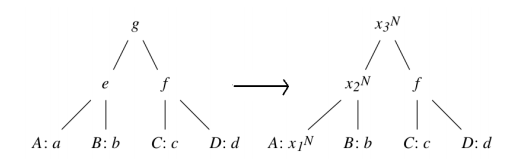
\includegraphics[scale=1]{Update-tree}
\caption{Thay đổi Key trong Ratchet tree}

{Sự thay đổi của nhóm trong Ratchet tree do A cập nhật khóa với các node secret x$_{1}^{N}$, x$_{2}^{N}$, x$_{3}^{N}$ từ lá đến gốc. Ở đây chúng tôi hiển thị cây node secret. Hãy nhớ lại rằng người dùng biết các bí mật của nút trên đường dẫn lá Lá của họ đến thư mục gốc, nhưng họ biết các khóa chung cho tất cả các nút trong cây.}
\end{center}
\end{figure}

Xem [Hình ~\ref{fig:Update-message}] về một ví dụ. Thông báo \gls{Update} chứa một khóa được mã hóa cho mỗi nút trên copath của lá người dùng cập nhật, do đó có kích thước \textit{O(log$_{2}$(n))}.

\begin{figure}[!h]
\begin{center}
\label{fig:Update-message}
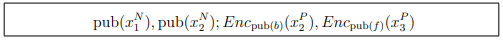
\includegraphics[scale=1]{Update-message}
\caption{Thông tin \gls{Update} tương ứng với bản cập nhật trong [Hình ~\ref{fig:Update-tree}].}
\end{center}
\end{figure}

Khi người dùng V nhận được thông báo \gls{Update} này, V sẽ sử dụng nó để cập nhật bản sao của cây ratchet của mình như sau:

\begin{itemize}
	\item{V đặt các khóa chung cho các nút trên đường dẫn trực tiếp của A  đến các nút được đưa ra trong phần (1) của thông báo \gls{Update}}
	\item{V giải mã bí mật đường dẫn cập nhật cho nút tổ tiên chung gần nhất M của nó với U, tức là, nút gần nhất là tổ tiên của cả hai lá U và V, từ một trong các giá trị được mã hóa được đưa ra trong phần (2) của thông báo \gls{Update}. Điều này là có thể bởi vì theo định nghĩa về độ phân giải của nút, U đã gửi bí mật đường dẫn của M được mã hóa dưới khóa chung K của một số nút trên đường đi giữa lá V và M. V biết khóa riêng tư tương ứng với K, do đó có thể giải mã bí mật đường dẫn của M. Trong ví dụ của [Hình ~\ref{fig:Update-tree}], tổ tiên chung gần nhất của B với A là cha mẹ của chúng và B có thể giải mã x$_{2}^{P}$ bằng cách sử dụng priv(b). Tổ tiên chung gần nhất của mỗi C và D với A là gốc và C và D có thể giải mã x$_{3}^{P}$ bằng cách sử dụng priv(\textit{f}).}
	\item{V tính toán các bí mật đường dẫn cập nhật cho tất cả tổ tiên của M, sử dụng \acrshort{kdf} và sau đó tính toán các node secret tương ứng bằng cách sử dụng \acrshort{kdf}.}
\end{itemize}

\begin{figure}[!h]
\begin{center}
\label{fig:Update-copath}
\caption{đưa ra một ví dụ minh họa quá trình này}
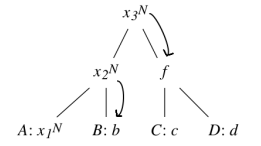
\includegraphics[scale=1]{Update-copath}

{Một minh họa về cách thông báo \gls{Update} TreeKEM trong [Hình ~\ref{fig:Update-message}] hoạt động, tức là cách nó thông báo cho những người dùng khác về những bí mật mới. Nó gửi (tiền thân x$_{2}^{P}$) của x$_{2}^{N}$ đến B bằng cách mã hóa nó dưới pub(b), trong khi nó gửi (tiền thân x$_{3}^{P}$) của x$_{3}^{N}$ đến C và D bằng cách mã hóa nó dưới pub(f).}
\end{center}
\end{figure}

Quan sát rằng giao thức cập nhật khóa: mỗi người dùng biết tất cả các bí mật nút trên đường dẫn lá Lá của họ đến gốc, cũng như tất cả các khóa công khai trong cây, nhưng họ không thể tính toán các bí mật nút khác trong cây


\subsection{Init and Application Secrets}
Mục đích của TreeKEM là tạo ra các bí mật được chia sẻ bởi tất cả các thành viên trong nhóm, sau đó họ có thể sử dụng để lấy các khóa mã hóa tin nhắn. Để thực hiện điều này, TreeKEM sử dụng các bí mật nút gốc để tạo ra một chuỗi các bí mật init, kết hợp hoàn toàn các bí mật nút gốc từ tất cả các bản cập nhật trước đó. Bí mật ban đầu sau đó được kết hợp với thông tin trạng thái nhóm để tạo bí mật ứng dụng, được sử dụng để tạo khóa mã hóa tin nhắn thực tế. [Hình ~\ref{fig:init}] cho thấy quá trình này theo sơ đồ. Kết hợp các bí mật gốc cũ và thông tin trạng thái nhóm vào các khóa là cần thiết để cung cấp bảo mật sau thỏa hiệp và tính nhất quán của người tham gia.

\begin{figure}[!h]
\begin{center}
\label{fig:init}
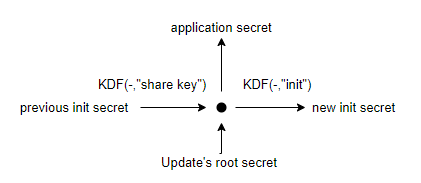
\includegraphics[scale=1]{init}
\caption{Cập nhật khóa chung}
{Lấy bí mật ứng dụng mới sau thông báo Cập nhật TreeKEM, sử dụng chuỗi bí mật init để kết hợp bí mật nút gốc từ tất cả các thay đổi trạng thái trước đó.}
\end{center}
\end{figure}


\subsection{Adding and Removing Users}
Giả sử người dùng U muốn xóa người dùng V khỏi nhóm. Để làm điều này, họ phải chia sẻ một bí mật mới với tất cả người dùng ngoại trừ V, mọi người dùng ngoại trừ V sau đó sử dụng để lấy bí mật ứng dụng mới. Bằng cách đó, V không thể giải mã tin nhắn trong tương lai được gửi đến nhóm.

TreeKEM thực hiện điều này như sau. Đối với người dùng U để xóa người dùng V, họ tạo một thông báo \gls{Remove}, chứa định danh V và thông báo \gls{Update} được gửi như thể U đang ở vị trí của V trên cây. Mọi người dùng ngoại trừ V đều lấy được bí mật nút gốc mới từ bản cập nhật này và sử dụng nó để lấy bí mật ứng dụng và init mới. Sau đó, mọi người dùng đặt lại tất cả các node secret trên đường dẫn trực tiếp của V.Cuối cùng đối với nút có cùng cha mẹ với V sẽ được đặt thành cha mẹ của chúng. Xem [Hình ~\ref{fig:Remove-tree}] cho một ví dụ.

\begin{figure}[!h]
\begin{center}
\label{fig:Remove-tree}
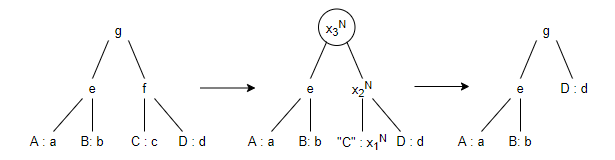
\includegraphics[scale=1]{Remove-tree}
\caption{Remove user}
{Xóa người dùng trong TreeKEM. Ở đây A loại bỏ C với các bí mật nút cập nhật x$_{1}^{N}$, x$_{2}^{N}$, x$_{3}^{N}$. Bí mật nút gốc được khoanh tròn, x$_{3}^{N}$, được sử dụng để tạo bí mật ứng dụng và init mới mà C.}
\end{center}
\end{figure}

Đối với người dùng U để thêm người dùng V, họ gửi thông điệp tới V chứa trạng thái nhóm hiện tại và cây khóa công khai và bí mật init gần đây nhất. Sau đó, bạn gửi một tin nhắn Thêm cho cả nhóm, bao gồm V, trong đó có khóa công khai cho V. Mọi người dùng sau đó:

\begin{itemize}
	\item{Điều chỉnh cấu trúc cây để chứa một chiếc lá mới cho V trong khi giữ cho nó cân bằng trái.}
	\item{Xuất phát các bí mật init và ứng dụng mới từ bí mật init hiện tại như trong [Hình ~\ref{fig:init}], sử dụng một chuỗi các số 0 thay cho bí mật nút gốc cập nhật}
\end{itemize}

Cuối cùng, V đặt bí mật nút lá riêng của mình thành bí mật được sử dụng để lấy khóa công khai. Người ta cho rằng một mình V biết bí mật nút này. Xem [Hình ~\ref{fig:Add-tree}] cho một ví dụ:

\begin{figure}[!h]
\begin{center}
\label{fig:Add-tree}
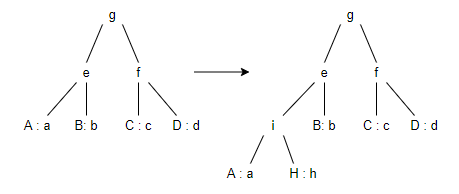
\includegraphics[scale=1]{Add-tree}
\caption{Add user}
{Thêm người dùng trong TreeKEM. Ở đây A thêm H với bí mật nút lá ban đầu h.}
\end{center}
\end{figure}

Lưu ý rằng sau khi xử lý các thông báo \acrshort{Add}, V biết tất cả các khóa chung, tất cả các bí mật nút trên đường dẫn trực tiếp của nó (cụ thể là bí mật nút lá) và bí mật ứng dụng và init mới. Do đó V có thể hoạt động như một thành viên nhóm.


\end{document}